%****************************************************************%
% FILE: intro.tex                                                %
% CONTENTS :                                                     %
% introduzione generale sull'argomento trattato nel documento    %
% azienda, cliente, progetto, metodologia lavoro                 %
% cosa contiene il resto della tesi                              %
%****************************************************************%
\documentclass[./main.tex]{subfiles}

\begin{document}
Questa tesi si occupa di analizzare lo sviluppo, dall'architettura sottostante al prodotto presentato agli utenti, di un'applicazione mobile realizzata durante il periodo di stage dell'autrice, svolto presso l'azienda Elan42. L'applicazione è commissionata dall'Istituto di Scienze Marine del Consiglio Nazionale delle Ricerche (ISMAR-CNR), un ente pubblico esterno all'azienda.

% img logo elan42 %
\begin{figure}[!ht]
\vspace{1cm}
\centering

\includegraphics[width=3cm]{images/logo_elan42.pdf}
\caption{Logo Elan42}
\label{fig:elan42}
\end{figure}

\textbf{Elan42} è una Digital Agency -- \textit{agenzia digitale} -- con sede a Venezia. Essa fornisce servizi di hosting di alta qualità promuovendo alternative sostenibili con lo scopo di ridurre l'inquinamento digitale. Inoltre si occupa della realizzazione di siti web professionali. Elan42 reputa fondamentale il concetto di codice aperto -- \textit{open source} -- come strumento di condivisione, conoscenza e trasparenza\footcite[\url{https://www.elan42.com/}]{website-elan42}.\par

\begin{quote}
\textit{Il software open-source differisce dagli altri software perché ha un contratto di licenza meno restrittivo: invece di utilizzare una licenza restrittiva che impedisce di modificare il programma o condividerlo, ne viene incoraggiata la condivisione e la modifica del software.  Chiunque lo desideri può distribuire, modificare o addirittura creare opere derivate basate su quel codice sorgente\footcite[\url{https://web.archive.org/web/20081028104313/http://www.diffingo.com/oss/whyoss}]{website-whatis-opensource}. Quindi no, open-source non significa solo che si ha libero accesso al codice sorgente\footcite[\url{https://web.archive.org/web/20070611152544/https://opensource.org/docs/osd}]{website-opensource-def}}.
\end{quote} 

Un aspetto interessante è che Elan42 si rende disponibile alla realizzazione di vari progetti, anche se essi si collocano al di fuori dal proprio ambito specialistico. In particolare, il progetto che verrà discusso nel presente documento, ideato e commissionato da un cliente esterno all'agenzia, presenta un argomento non conforme a quelli tipici dell'azienda.\par

% img logo cnr %
\begin{figure}[!ht]
\vspace{1cm}
\centering

\includegraphics[width=5cm]{images/logo_cnr.pdf}
\caption{Logo ISMAR-CNR}
\label{fig:cnr}
\end{figure}

\textbf{ISMAR-CNR} è il cliente che ha commissionato il progetto trattato. Esso rappresenta la più grande istituzione italiana che si occupa dello sviluppo scientifico nel campo della scienza dell'oceano\footcite[\url{https://www.ismar.cnr.it/}]{website-ismar-cnr}.\par

Il \textbf{progetto} consiste nello sviluppo di un'applicazione come nuova progettazione di una precedentemente creata\footcite[\url{https://www.ismar.cnr.it/terza-missione/app/\#2}]{website-ismar-cnr} ormai obsoleta e non più funzionante, che consenta la visualizzazione di dati meteorologici forniti da ISMAR-CNR.\par

L'applicazione raccoglie i dati da stazioni, radar e satelliti. Queste sorgenti di dati rappresentano il cuore dell'applicazione, senza i dati l'applicazione non può esistere. Un problema che comprometterà il processo evolutivo del software, nonché della tesi stessa, è il fatto che non sempre questi dati risultano disponibili. In particolare alcuni di essi sono gestiti da enti privati che non permettono l'utilizzo dei dati raccolti. Quando i dati sono disponibili vengono elaborati e inviati al lato grafico dell'applicazione che li visualizza in base alle esigenze dell'utente finale. Tutto questo lavoro viene supportato da politiche di riuso del codice che consentono di creare modelli generali per l'importazione dei dati e per l'invio e la visualizzazione di essi. Inoltre un database locale aiuta nella memorizzazione delle informazioni per rendere efficiente l'accesso ai dati da parte dell'applicazione mobile.\par 

Una volta terminata, l'applicazione entrerà finalmente in produzione e, al rilascio della prima versione, sarà utilizzabile da qualsiasi utente. Essa infatti si rivolge sia a un pubblico generale ma anche, in una certa misura, a un pubblico più specializzato ed esperto. Questo perché alcuni dati trattati sono utili nella vita quotidiana (per es. temperatura e vento) altri invece non sono di particolare interesse al di fuori dell'ambito specialistico (per es. clorofilla). Infine l'applicazione dovrà funzionare sia su sistemi Android che Apple iOS (desktop, mobile e tablet, dando precedenza alla versione mobile) e dovrà essere scaricabile dai rispettivi negozi online.\par

Da ora in avanti ci si riferirà all'applicativo creato equivalentemente con i termini \textit{Ismar Data}, \textit{applicazione}, e \textit{progetto}.

\paragraph{Metodologia di lavoro.} L'applicazione è sviluppata da un team. Quando un gruppo di persone deve collaborare per portare a termine un compito, occorre stabilire il metodo con il quale si lavora.\par

Il modo tradizionale di sviluppare un progetto software è il modello \textbf{waterfall}. Esso consiste nella suddivisione in rigide fasi svolte in sequenza; quando una fase finisce, inizia la successiva. Non consentendo agli sviluppatori di tornare indietro e rivedere le fasi già concluse (da qui il nome waterfall - \textit{cascata} - )\footcite[131]{CONRAD2011129}. L'alternativa più innovativa, nonché quella utilizzata per il progetto, è il \textbf{metodo agile}\footnote{Il termine agile è pronunciato all'inglese.}. Esso consente una gestione del progetto in un modo collaborativo, nel quale il team consegna il prodotto a piccoli passi, dando la possibilità al cliente di effettuare cambiamenti. Inoltre permette di fermarsi e tornare alle fasi precedenti qualora si presenti la necessità di effettuare miglioramenti\footcite[7]{waters2012all}. In realtà la metodologia agile è un insieme di valori e principi descritti nel manifesto redatto da K. Beck et al\footcite{beck2001manifesto}. Ogni metodo che segue quei fondamenti è ritenuto agile\footcite[10]{waters2012all}.

\begin{figure}[!ht]
\noindent\begin{minipage}{0.6\textwidth}
\vspace{1cm}
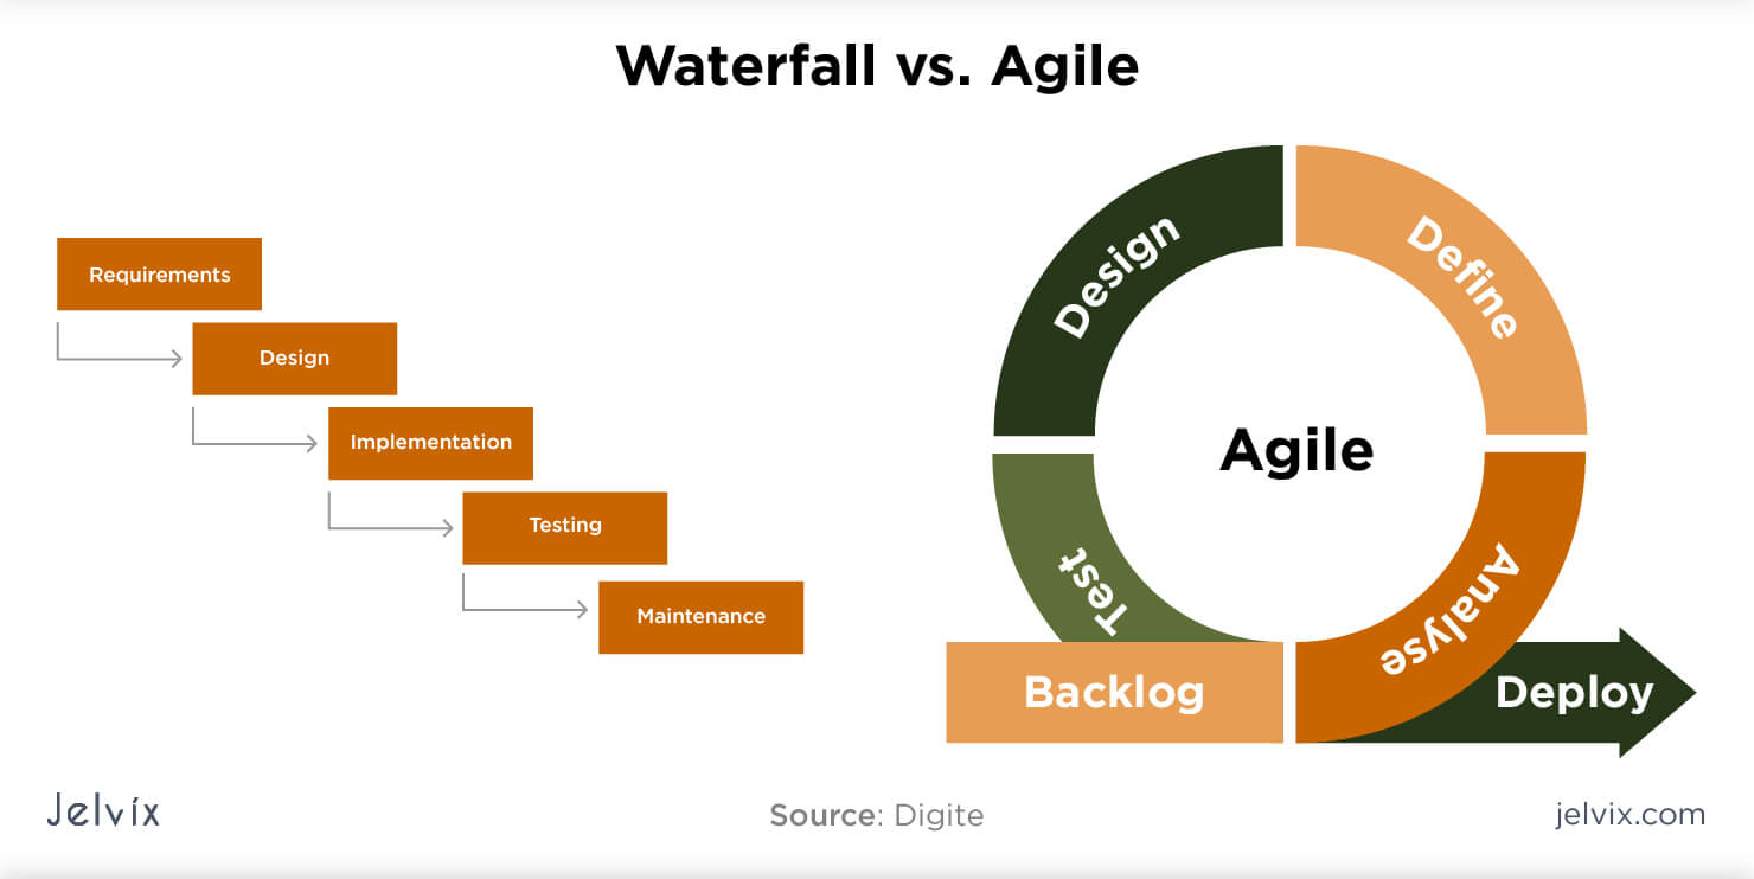
\includegraphics[width=\textwidth]{images/waterfall-vs-agile.pdf}
\captionsetup{font=small, hypcap=false}
\captionof{figure}{Waterfall vs. Agile\footcite[Fonte: ][]{img-waterfall-vs-agile}.}
\label{fig:waterfall_vs_agile}
\end{minipage}
\hspace{0.05\textwidth}
\begin{minipage}{0.3\textwidth}
\begin{small}
Confronto grafico tra le due filosofie di lavoro, \textit{waterfall} a sinistra e \textit{agile} a destra. Si può notare come il metodo \textit{agile} risulta essere più flessibile e quindi più adatto allo sviluppo di un software.
\end{small}
\end{minipage}
\vspace{0.25cm}
\end{figure}

In particolare, nello sviluppo di \textit{Ismar Data}, il framework che si adatta meglio alla situazione è \textbf{scrum}. È importante osservare che, data l'imprevedibilità e la poca certezza presente nello sviluppo dell'applicazione dovuto al problema della mancanza dei dati, il metodo descritto non viene applicato alla lettera. Il metodo scrum si basa su cinque valori fondamentali: \blockquote{\textit{Impegno, Focus, Apertura, Rispetto e Coraggio}}\footcite[4]{scrum-guide-ita}. Il lavoro viene suddiviso in \blockquote{\textit{sprint}} della durata di due settimane, durante le quali ogni sviluppatore -- \textit{developer}\footcite[5-6]{scrum-guide-ita} -- svolge il compito che gli è stato assegnato. I compiti sono prelevati da un \blockquote{\textit{backlog\footcite[11]{scrum-guide-ita}}}, una lista contenente tutte le richieste del cliente in ordine di importanza. Non è detto che vengano effettivamente implementate tutte le funzionalità richieste, sopratutto nelle prime versioni dell'applicazione.\par

La gestione dei compiti viene fatta utilizzando l'applicativo \textbf{Asana}\footcite[\url{https://asana.com/it}]{website-asana}. Esso è uno strumento di gestione del lavoro che, grazie alle sue funzionalità di coordinazione del team e monitoraggio delle attività\footcite[\url{https://help.asana.com/hc/it/articles/14250783001627-Come-iniziare-a-usare-Asana\#h\_01HEQV7CDGXHBY06W9PQAXB8RK}]{website-asana}, facilita l'utilizzo del metodo scrum.\par

\paragraph{Perché continuare a leggere?} I successivi capitoli analizzeranno l'applicazione, dando particolare rilevo alla descrizione delle sorgenti di dati e all'architettura sottostante, con un'attenzione alle problematiche presenti e alle possibili soluzioni. Ulteriore spazio sarà dato allo sviluppo concreto del progetto, esaminando nel dettaglio gli strumenti utilizzati, sia per la comunicazione che per la produzione, le funzionalità implementate e la gestione dei dati disponibili. Infine si trarranno le conclusioni sull'intero percorso, verificando se l'obiettivo è stato raggiunto oppure se qualcosa non ha funzionato come avrebbe dovuto.
Quindi, ci si trova davanti ad una scelta: andare avanti o restare fermi. Andare avanti non sempre significa arrivare al traguardo, ma l'importante è provarci anche se ad ogni passo avanti ne corrispondono due indietro.\par

\end{document}